% !TEX program = XeLaTeX
% -----------------------------------------------------------------------------
% The Core Principles of Onri Jay Benally
% A Beamer deck designed for XeLaTeX + IBM Plex fonts.
% -----------------------------------------------------------------------------
\documentclass[presentation,aspectratio=169,11pt]{beamer}

% ---------- Font setup: IBM Plex ----------
\usepackage{fontspec}
\defaultfontfeatures{Ligatures=TeX, Scale=MatchLowercase}
% IBM Plex is preferred (as installed by the user). Fallbacks keep the deck compilable
% on systems that do not have IBM Plex installed.
\IfFontExistsTF{IBM Plex Sans}{
  \setsansfont{IBM Plex Sans}[Scale=MatchLowercase, Ligatures=TeX]
}{
  % TeX distributions vary. These fallbacks keep compilation reliable.
  \IfFontExistsTF{Noto Sans}{
    \setsansfont{Noto Sans}[Scale=MatchLowercase, Ligatures=TeX]
  }{
    \setsansfont{DejaVu Sans}[Scale=MatchLowercase, Ligatures=TeX]
  }
}
\IfFontExistsTF{IBM Plex Mono}{
  \setmonofont{IBM Plex Mono}[Scale=MatchLowercase]
}{
  % As with sans fonts, prefer broadly available system monospace fonts for fallbacks.
  \IfFontExistsTF{Noto Sans Mono}{
    \setmonofont{Noto Sans Mono}[Scale=MatchLowercase]
  }{
    \setmonofont{DejaVu Sans Mono}[Scale=MatchLowercase]
  }
}
\renewcommand\familydefault{\sfdefault}

% ---------- Math ----------
% XeLaTeX defaults to Computer Modern math. If you prefer an OpenType math font
% (e.g., STIX Two Math), you can re-enable unicode-math here.

% ---------- Layout safety (avoid overfull lines) ----------
\usepackage{ragged2e}
\setlength{\emergencystretch}{2.5em}
\sloppy

% Keep content inside frame margins.
\setbeamersize{text margin left=0.85cm, text margin right=0.85cm}

% ---------- Theme + visual system (minimal, readable) ----------
\usetheme{Boadilla}
\setbeamertemplate{navigation symbols}{}

\usepackage{xcolor}
\definecolor{OnriNavy}{HTML}{0B1F3B}
\definecolor{OnriBlue}{HTML}{001D6C}
\definecolor{OnriSand}{HTML}{F3EFE2}
\definecolor{OnriCharcoal}{HTML}{2A2A2A}

\setbeamercolor{structure}{fg=OnriBlue}
\setbeamercolor{normal text}{fg=OnriCharcoal,bg=white}
\setbeamercolor{frametitle}{fg=OnriNavy,bg=white}
\setbeamercolor{block title}{fg=white,bg=OnriNavy}
\setbeamercolor{block body}{fg=OnriCharcoal,bg=OnriSand}

% Footline with slide numbers (kept compact)
\setbeamertemplate{footline}{%
  \leavevmode%
  \hbox{%
    \begin{beamercolorbox}[wd=.78\paperwidth,ht=2.3ex,dp=1.0ex,leftskip=0.85cm,rightskip=0.85cm]{author in head/foot}%
      \usebeamerfont{author in head/foot}\insertshorttitle
    \end{beamercolorbox}%
    \begin{beamercolorbox}[wd=.22\paperwidth,ht=2.3ex,dp=1.0ex,center]{date in head/foot}%
      \usebeamerfont{date in head/foot}\insertframenumber{} / \inserttotalframenumber
    \end{beamercolorbox}%
  }%
  \vskip0pt%
}

% ---------- Math, tables, graphics ----------
\usepackage{amsmath, amsfonts, amssymb, mathtools}
\usepackage{tabularx}
\usepackage{booktabs}
\usepackage{tikz}
\usetikzlibrary{calc, positioning, arrows.meta}
\usepackage{dirtree}

% Beamer text helpers
\newcommand{\KeyTerm}[1]{\textbf{#1}}

% ---------- Title data ----------
\title[Core Principles]{The Core Principles of Onri Jay Benally}
\subtitle{Self-sufficiency, de-nuancing, strategy, and proactive optimism}
\author{Onri Jay Benally}
\date{\today}

\begin{document}

% -----------------------------------------------------------------------------
\begin{frame}[plain]
  \titlepage
\end{frame}

% -----------------------------------------------------------------------------
\begin{frame}{Orientation and intent}
\justifying
Through repeated engineering work (hardware, software, and human coordination), these principles are framed as a kind of actionable playbook, where ideas are progressively compressed into decisions, checklists, and validated procedures.

\vspace{0.75em}
\begin{block}{}
\justifying
By starting with information gathering (raw data compilation), and then by iterating through de-nuancing, the work product increasingly behaves like a stable control law: it becomes clearer, more testable, and more transferable.
\end{block}
\end{frame}

% -----------------------------------------------------------------------------
\begin{frame}{Overview of the four core principles (1/2)}
\justifying
\begin{table}
\scriptsize
\begin{tabularx}{\linewidth}{@{}l X X@{}}
\toprule
\textbf{Principle} & \textbf{Working definition} & \textbf{Observable test}\\
\midrule
\KeyTerm{Self-sufficiency} & By design, the system (or team) relies on local capabilities, clear interfaces, and reproducible toolchains. & By measuring time-to-rebuild, dependency count, single-point-of-failure count, and recovery time after perturbations.\\
\addlinespace
\KeyTerm{De-nuancing} & By iteration, nuance becomes explicit assumptions, and then becomes a smaller set of sharp claims that guide decisions. & By tracking ambiguity sources, and then by validating that decisions remain consistent across contexts and stakeholders.\\
\bottomrule
\end{tabularx}
\end{table}
\end{frame}

\begin{frame}{Overview of the four core principles (2/2)}
\justifying
\begin{table}
\scriptsize
\begin{tabularx}{\linewidth}{@{}l X X@{}}
\toprule
\textbf{Principle} & \textbf{Working definition} & \textbf{Observable test}\\
\midrule
\KeyTerm{Strategy} (data-first) & By first compiling raw data, and then by selecting objectives and constraints, the plan becomes an algorithm, instead of a story. & By verifying that inputs, objectives, and constraints are documented, and then by running a repeatable decision procedure.\\
\addlinespace
\KeyTerm{Proactive optimism} (performance-based) & By measuring improvement loops, optimism becomes a policy: it selects actions that increase capability, resilience, and clarity. & By demonstrating sustained leading-indicator improvement (throughput, yield, mean-time-between-failure, decision latency).\\
\bottomrule
\end{tabularx}
\end{table}
\end{frame}

% -----------------------------------------------------------------------------
\section{Self-sufficiency}

\begin{frame}{Principle 1: Self-sufficiency}
\justifying
Through tools, skills, and documentation that stay close to the work, you increasingly rely on yourself (and on your immediate collaborators) rather than on fragile external dependencies.

\vspace{0.6em}
Through modular architecture, reproducible environments, and explicit interfaces, one increases autonomy, and then lowers coordination overhead, while raising resilience under supply-chain, compute, and personnel shocks.

\vspace{0.8em}
\begin{block}{Engineering translation}
\justifying
By treating every dependency as a potential failure mode, it progressively converts them into either (i) a locally reproducible capability, (ii) a constrained interface with a fallback, or (iii) an explicitly accepted risk with monitoring.
\end{block}
\end{frame}

\begin{frame}{Self-sufficiency as a systems property}
\justifying
\begin{itemize}
  \item \KeyTerm{Toolchain autonomy:} build scripts, firmware images, simulation notebooks, and test procedures that rerun on demand.
  \item \KeyTerm{Material autonomy:} qualified substitutes, parametric drawings, and process windows that remain valid under vendor variation.
  \item \KeyTerm{Cognitive autonomy:} decision logs, assumption registers, and minimal handoff documentation that lowers tribal knowledge.
  \item \KeyTerm{Failure-aware design:} graceful degradation, redundancy where it pays, and instrumentation where it predicts.
\end{itemize}

\vspace{0.4em}
\begin{block}{Useful linguistic connection (etymology)}
\justifying
\emph{Autarky} (Greek \emph{autarkeia}, self-sufficiency) historically describes a polity, while engineering self-sufficiency reinterprets it as a reproducible capability boundary.
\end{block}
\end{frame}

% -----------------------------------------------------------------------------
\section{De-nuancing}

\begin{frame}{Principle 2: De-nuancing}
\justifying
Through careful discussion, a confusing topic becomes a clear set of decisions, and then it becomes a teachable procedure.

\vspace{0.6em}
Through iterative model reduction (where hidden assumptions are surfaced, and then where uncertainty is bounded), the topic compresses into an explicit operating envelope, where actions remain consistent with objectives.

\vspace{0.8em}
\begin{block}{A practical de-nuancing loop}
\justifying
By listing sources of ambiguity, and then by choosing a measurement or a test, and then by writing the smallest decision rule that passes that test, one reduces nuance while increasing shared clarity.
\end{block}
\end{frame}

\begin{frame}{On de-nuancing}
\justifying
\small
\begin{quote}
I am of the opinion, which is very strong, that nuance, when applied to a topic, should never remain nuanced forever. The nuance should progressively diminish, ideally to zero, as the ultimate goal, although the realistic goal is slightly less than the true ideal, which is fine. Thus, it becomes clarified and straightforward, with clear instruction that enables clear decisions and applications when relevant. If something remains nuanced perpetually, then clearly there is a kind of laziness or intellectual laziness that needs to be addressed, as well as an acknowledgment of the next steps to be taken and a highlight of what was overlooked for full transparency and proactivity. I think this is key to human-to-human interaction being successful and to long-term social stability.
\end{quote}
\vspace{0.35em}
\hfill\textit{--- Onri Jay Benally (2025)}
\end{frame}

\begin{frame}{When ``nuance goes to zero'' becomes true (by design)}
\justifying
In open-ended reality, nuance stays present because the system has unbounded contexts, and because stakeholders optimize different objectives. Through deliberate restriction and explicit assumptions, the de-nuancing goal becomes achievable.

\vspace{0.75em}
\begin{block}{Making ``zero nuance'' effectively true}
\justifying
\begin{enumerate}
  \item \KeyTerm{Scope restriction:} define a bounded operating envelope (inputs, outputs, constraints), so ambiguity loses room to hide.
  \item \KeyTerm{Assumption closure:} write assumptions as first-class objects (versioned), so disagreement becomes traceable.
  \item \KeyTerm{Decision compilation:} convert discussion into an executable policy (checklist, rubric, test, or optimization), so interpretation becomes repeatable.
\end{enumerate}
\end{block}

\vspace{0.5em}
\small
Once these operations are applied, the topic changes identity: it becomes an \emph{assumption-closed operating procedure} rather than a perpetually interpretive conversation.
\end{frame}

\begin{frame}{De-nuancing as information compression (a research bridge)}
\justifying
Through summarizing, one keeps the parts that matter for the decision, and then removes the rest.

\vspace{0.6em}
Through an explicit compression objective, one searches for a representation $T$ of observations $X$ that preserves relevance to a target $Y$.

\vspace{0.6em}
\begin{block}{One formal lens: the Information Bottleneck objective}
\justifying
\vspace{-0.5em}
$$
\min_{p(t\mid x)}\; I(X;T)\; -\; \beta\, I(T;Y)
$$
\vspace{-0.2em}
\small
Here, $I(\cdot;\cdot)$ denotes mutual information, and $\beta$ tunes the compression versus relevance tradeoff.
\end{block}

\vspace{0.3em}
\footnotesize
A canonical open-access reference is Tishby, Pereira, and Bialek (2000), \href{https://arxiv.org/abs/physics/0004057}{arXiv:physics/0004057}.
\end{frame}

% -----------------------------------------------------------------------------
\section{Strategy (data-first)}

\begin{frame}{Principle 3: Strategy (starting with raw data)}
\justifying
Through collecting facts first, one lowers confusion, and then raises the quality of decisions.

\vspace{0.6em}
Through data compilation, and then through hypothesis management, strategy can be turned into an inference-and-control loop, where uncertainty shrinks by design.

\vspace{0.8em}
\begin{block}{A disciplined ordering}
\justifying
By placing information gathering before opinion, and then by placing explicit objectives before tactics, the plan becomes less emotional, more measurable, and more resilient under surprise.
\end{block}
\end{frame}

\begin{frame}{Strategy as a pipeline (from data to action)}
\centering
\resizebox{0.98\linewidth}{!}{%
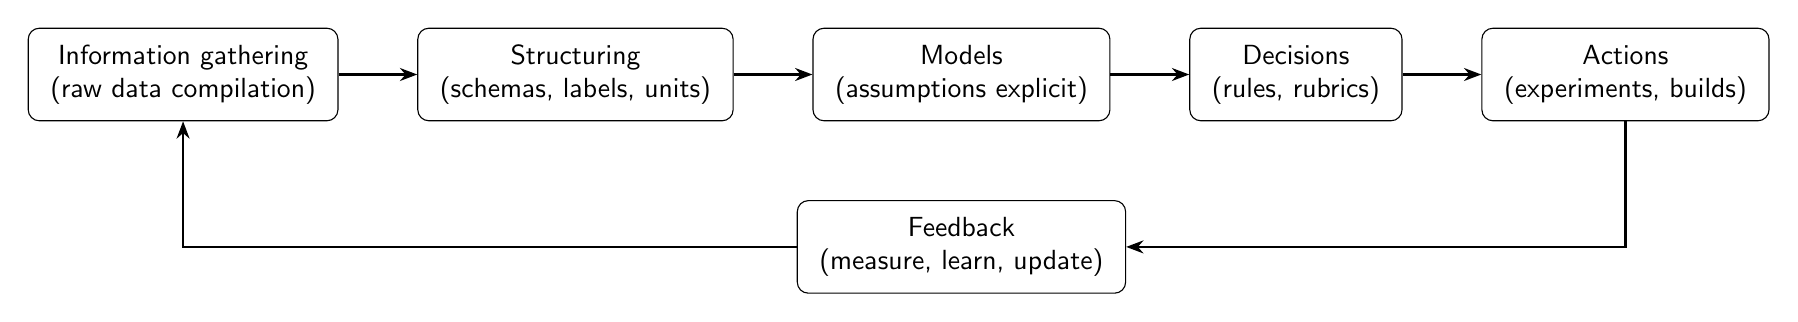
\begin{tikzpicture}[
  font=\sffamily,
  node distance=10mm,
  box/.style={draw, rounded corners, align=center, inner xsep=8pt, inner ysep=6pt},
  arr/.style={-{Stealth[length=2.2mm]}, thick}
]
  \node[box] (data) {Information gathering\\(raw data compilation)};
  \node[box, right=of data] (structure) {Structuring\\(schemas, labels, units)};
  \node[box, right=of structure] (models) {Models\\(assumptions explicit)};
  \node[box, right=of models] (decide) {Decisions\\(rules, rubrics)};
  \node[box, right=of decide] (act) {Actions\\(experiments, builds)};

  \draw[arr] (data) -- (structure);
  \draw[arr] (structure) -- (models);
  \draw[arr] (models) -- (decide);
  \draw[arr] (decide) -- (act);

  \node[box, below=of models] (feedback) {Feedback\\(measure, learn, update)};
  \draw[arr] (act.south) |- (feedback.east);
  \draw[arr] (feedback.west) -| (data.south);
\end{tikzpicture}%
}

\vspace{0.6em}
\justifying
\small
Through this ordering, de-nuancing becomes a built-in compiler stage: it turns discussion into a smaller representation that still predicts outcomes.
\end{frame}

% -----------------------------------------------------------------------------
\section{Proactive optimism}

\begin{frame}{Principle 4: Proactive optimism (performance-based)}
\justifying
Through choosing actions that improve one's situation, optimism becomes a habit that is supported by evidence.

\vspace{0.6em}
Through selecting actions that maximize expected improvement under constraints, optimism becomes a control policy, where progress is tracked via leading indicators.

\vspace{0.75em}
\begin{block}{A compact quantitative phrasing}
\justifying
\vspace{-0.5em}
$$
 a^{\star} \in \arg\max_{a\in\mathcal{A}}\; \mathbb{E}\bigl[\Delta \mathcal{P}\mid a,\, D\bigr]\quad\text{subject to}\quad \text{risk}(a)\le r_{\max}
$$
\vspace{-0.2em}
\small
Here, $\mathcal{P}$ denotes a performance score (yield, latency, robustness), $D$ denotes the compiled evidence, and $r_{\max}$ encodes risk tolerance.
\end{block}
\end{frame}

\begin{frame}{Proactive optimism as a stability mechanism}
\justifying
\begin{itemize}
  \item By focusing on leading indicators, vague hope is converted into measurable progress.
  \item By running tight feedback loops, learning rate increases while reducing the need for rework.
  \item By maintaining a performance baseline, drift can be detected early, and it may be corrected cheaply.
  \item By designing for recovery (in addition to prevention), one raises overall resilience.
\end{itemize}

\vspace{0.6em}
\begin{block}{Direct conceptual bridge}
\justifying
In resilience engineering language, proactive optimism aligns with a shift from failure fixation toward success conditions, where performance variability becomes observable and steerable.
\end{block}
\end{frame}

% -----------------------------------------------------------------------------
\section{Orthogonality to Murphy's Law}

\begin{frame}{Concise aphorism}
\justifying
\Large
\begin{quote}
If one provides the right ingredients, applied in the right way, then the system of interest will solve its own self internally, no matter how complicated its mechanics are. It is likened to a perpendicular (orthogonal) relationship to that of Murphy's Law.\footnote{Murphy's Law is commonly summarized as: \emph{``anything that can go wrong, will go wrong.''}}\footnote{In engineering practice, Murphy's Law usefully highlights the inevitability of failure modes, and therefore it motivates instrumentation, redundancy, and disciplined risk management.}
\end{quote}
\end{frame}

\begin{frame}{Visual metaphor: orthogonality}
\centering
\resizebox{0.90\linewidth}{!}{%
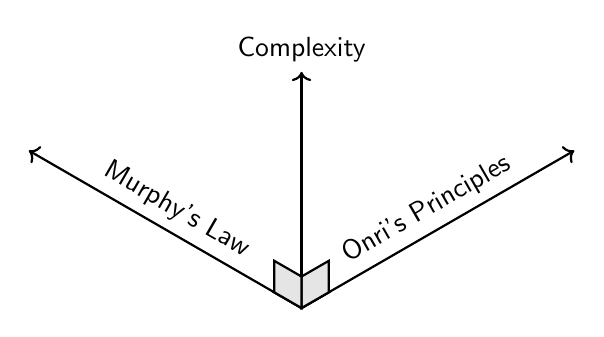
\begin{tikzpicture}[
  % Isometric projection
  x={(0.866cm,0.5cm)},
  y={(-0.866cm,0.5cm)},
  z={(0cm,1cm)},
  font=\sffamily,
  thick
]
  % Axes with sloped labels
  \draw[->] (0,0,0) -- (4,0,0) node[midway, above, sloped] {Onri's Principles};
  \draw[->] (0,0,0) -- (0,4,0) node[midway, above, sloped] {Murphy's Law};
  \draw[->] (0,0,0) -- (0,0,3) node[anchor=south] {Complexity};

  % Orthogonality markers (boxes) at the origin corners
  \draw[fill=gray!20] (0,0,0) -- (0.4,0,0) -- (0.4,0.4,0) -- (0,0.4,0) -- cycle;  % XY plane box
  \draw[fill=gray!20] (0,0,0) -- (0.4,0,0) -- (0.4,0,0.4) -- (0,0,0.4) -- cycle;  % XZ plane box
  \draw[fill=gray!20] (0,0,0) -- (0,0.4,0) -- (0,0.4,0.4) -- (0,0,0.4) -- cycle;  % YZ plane box
\end{tikzpicture}%
}
\end{frame}

\begin{frame}{Visual metaphor: orthogonality}
\justifying
\small
By choosing ingredients and interfaces that reduce coupling, one increasingly prevents failure modes from aligning with the main success pathway.

\vspace{0.6em}
In linear algebra terms, orthogonality expresses independence: for vectors $a$ and $b$, $a\cdot b = 0$ means that motion along $a$ leaves $b$ unchanged. In systems terms, one designs in such a way that common failure directions remain weakly projected onto the success direction, at least inside the basin where assumptions hold.

\vspace{0.8em}
\begin{block}{Practical implication}
\justifying
Through de-nuancing, one makes the basin explicit. Through strategy, one measures the dominant failure directions. Through self-sufficiency, one preserves the ability to redesign ingredients. Through proactive optimism, one iterates until the remaining risk budget matches the objective.
\end{block}
\end{frame}

% -----------------------------------------------------------------------------
\section{Mathematical formalization and intuition}

\begin{frame}{Mathematical formalization (stability under a chosen ingredient set)}
\justifying
\small
Let a dynamical system be
\[
    \dot{x}(t) \;=\; F\!\bigl(x(t),\theta\bigr),
    \qquad x(t)\in\mathbb{R}^n,\; \theta\in\Theta\subset\mathbb{R}^m.
\]

\vspace{0.75em}
\textbf{Onri's condition}
\[
  \boxed{\;
    \exists\,\theta^{\star}\in\Theta\;
    \text{s.t.}\;
    \forall\,x_0\in\mathcal{B},\;
    \lim_{t\to\infty} \operatorname{dist}\!\bigl(x(t;x_0,\theta^{\star}),\, G\bigr) = 0
  \;}
\]

\vspace{0.75em}
\begin{itemize}
  \setlength\itemsep{0.45em}
  \item $\theta^{\star}$: \emph{right ingredients}, a parameter set embedding stability (under assumed constraints).
  \item $\mathcal{B}$: basin of attraction, the region of initial conditions where the claim remains valid.
  \item $G$: goal set (equilibrium, limit cycle, correct output, specification satisfaction, and so on).
\end{itemize}
\end{frame}

\begin{frame}{Interpretation (mapped back to the four principles)}
\justifying
\begin{enumerate}
  \item \KeyTerm{Self-sufficiency:} the capability to propose, build, and validate candidate $\theta$ locally, while preserving reproducibility.
  \item \KeyTerm{De-nuancing:} the progressive reduction of ambiguity in $F$, $\Theta$, $\mathcal{B}$, and $G$, until assumptions become explicit and testable.
  \item \KeyTerm{Strategy:} the algorithm used to search for $\theta^{\star}$, starting from raw data and ending in validated decisions.
  \item \KeyTerm{Proactive optimism:} the commitment to running the search loop repeatedly, while tracking performance improvement, and while shrinking decision latency.
\end{enumerate}

\vspace{0.5em}
\small
Through this mapping, the aphorism becomes a methodology: it becomes a disciplined search for $\theta^{\star}$, together with a disciplined definition of when the claim applies.
\end{frame}

\begin{frame}{Visual intuition}
\centering
\resizebox{0.82\linewidth}{!}{%
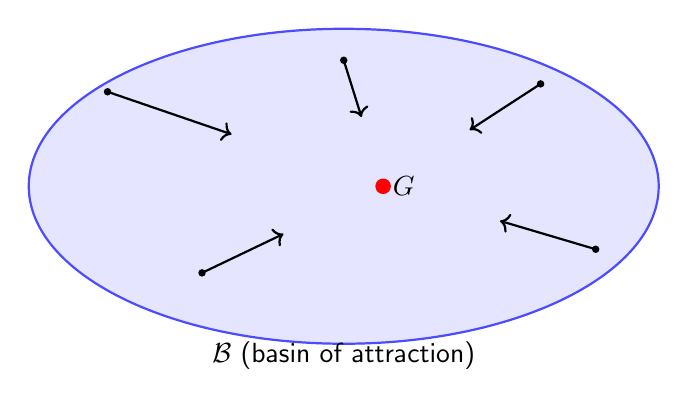
\begin{tikzpicture}
  % Basin of attraction ellipse
  \fill[blue!10] (0,0) ellipse (4cm and 2cm);
  \draw[blue!70, thick] (0,0) ellipse (4cm and 2cm);
  \node at (0,-2.15) {$\mathcal{B}$ (basin of attraction)};

  % Goal set point
  \filldraw[red] (0.5,0) circle (2.6pt);
  \node[right] at (0.5,0) {$G$};

  % Multiple starting points and arrows
  \foreach \x/\y in {-3/1.2, -1.8/-1.1, 2.5/1.3, 3.2/-0.8, 0/1.6}
    {
      \fill[black] (\x,\y) circle (1.35pt);
      \draw[->, thick] (\x,\y) -- ($(0.5,0)!0.55!(\x,\y)$);
    }
\end{tikzpicture}%
}
\end{frame}

\begin{frame}{Visual intuition (basin of attraction, reading)}
\justifying
\small
By choosing ingredients and constraints well, many different starting conditions still ``flow'' toward the same outcome.

\vspace{0.6em}
A basin of attraction $\mathcal{B}$ describes an operating envelope: inside it, the dynamics converge toward a goal set $G$. De-nuancing progressively specifies what counts as ``inside'' (assumptions, bounds, interfaces), while strategy supplies the measurements that confirm convergence.

\vspace{0.8em}
\begin{block}{Connection back to proactive optimism}
\justifying
By monitoring leading indicators, one can empirically map where $\mathcal{B}$ holds, and then it can be expanded by redesigning ingredients, interfaces, or feedback as needed.
\end{block}
\end{frame}


% -----------------------------------------------------------------------------
\section{Examples, connections, and language}

\begin{frame}{Practical examples}
\justifying
\begin{itemize}
  \item \KeyTerm{Proportional Integral Derivative (PID) control:} tuning gains so the closed-loop system stabilizes while it tracks targets.
  \item \KeyTerm{Software refactoring:} increasing cohesion and reducing coupling, so the codebase ``wants'' to remain correct under changes.
  \item \KeyTerm{Quantum error correction:} designing surface-code lattices so physical noise is pushed below a logical threshold.
  \item \KeyTerm{Ecosystem engineering:} altering constraints so predator--prey dynamics settle into sustainable regimes.
  \item \KeyTerm{Manufacturing yield:} reducing latent defect channels through measurement, process windows, and root-cause closure.
\end{itemize}
\end{frame}

\begin{frame}{Classification of direct and indirect connections, 1/2}
\justifying
\scriptsize
\dirtree{%
.1 The Core Principles of Onri Jay Benally.
.2 Self-sufficiency.
.3 Reproducible toolchains (build, test, document).
.3 Dependency minimization (fallbacks, substitutes).
.3 Resilience engineering (recovery, robustness).
.2 De-nuancing.
.3 Assumption registers (explicit, versioned).
.3 Model reduction (coarse-graining, sufficient statistics).
.3 Decision hygiene (rubrics, checklists).
}
\end{frame}

\begin{frame}{Classification of direct and indirect connections, 2/2}
\justifying
\scriptsize
\dirtree{%
.1 The Core Principles of Onri Jay Benally (continued).
.2 Strategy (data-first).
.3 Information gathering (raw data compilation).
.3 Hypothesis management (evidence, updates).
.3 Optimization (objectives, constraints).
.2 Proactive optimism (performance-based).
.3 Leading indicators (metrics that predict outcomes).
.3 Feedback loops (measure, learn, update).
}
\end{frame}


\begin{frame}{Classification of figures, fields, and historical lineage}
\justifying
\footnotesize
\dirtree{%
.1 Some intellectual and technical lineages.
.2 Cybernetics (steering, regulation).
.3 Norbert Wiener (feedback as a scientific language).
.3 William Ross Ashby (homeostasis, requisite variety).
.2 Information theory (measurement of uncertainty).
.3 Claude Shannon (communication limits, entropy).
.3 Information Bottleneck (relevance-preserving compression).
.2 Statistical physics and model reduction.
.3 Renormalization Group (coarse-graining across scales).
.2 Non-equilibrium thermodynamics.
.3 Ilya Prigogine (dissipative structures).
.2 Computation and self-organization.
.3 John von Neumann (automata, self-reproduction).
}
\end{frame}

\begin{frame}{Portmanteaus and etymologies}
\justifying
\small
\begin{table}
\begin{tabularx}{\linewidth}{@{}l X@{}}
\toprule
\textbf{Term} & \textbf{Linguistic roots, plus an engineering reading}\\
\midrule
\KeyTerm{De-nuancing} & Prefix \emph{de-} (removal, reversal) + \emph{nuance} (French, ``a shade''). In practice, it is an iterative removal of interpretive degrees of freedom, while preserving decision-relevant structure.\\
\addlinespace
\KeyTerm{Orthogonal} & Greek \emph{orthos} (straight) + \emph{gonia} (angle). In practice, it encodes independent design axes, where progress along one axis avoids trading away another.\\
\addlinespace
\KeyTerm{Strategy} & Greek \emph{strategos} (generalship). In practice, it becomes an algorithm for allocating limited resources under uncertainty.\\
\addlinespace
\KeyTerm{Cybernetics} & Greek \emph{kybern\=et\=es} (steersman). In practice, it becomes the language of feedback, regulation, and goal-seeking dynamics.\\
\bottomrule
\end{tabularx}
\end{table}
\end{frame}

\begin{frame}{Acronym glossary}
\justifying
\scriptsize
\begin{table}
\begin{tabularx}{\linewidth}{@{}l l X@{}}
\toprule
\textbf{Acronym} & \textbf{Expansion} & \textbf{Where it appears}\\
\midrule
PID & Proportional Integral Derivative & Control example; a concrete instance of shaping dynamics toward $G$.\\
IB & Information Bottleneck & De-nuancing as relevance-preserving compression of complex observations.\\
RG & Renormalization Group & Multi-scale de-nuancing, where coarse-graining yields simpler, predictive descriptions.\\
MSM & Markov State Model & Example of compressing dynamics into a lower-dimensional state representation.\\
MTBF & Mean Time Between Failures & Proactive optimism metric; tracks reliability improvement over time.\\
\bottomrule
\end{tabularx}
\end{table}
\end{frame}

% -----------------------------------------------------------------------------
\section{References}

\begin{frame}{References}
\justifying
\footnotesize
\begin{itemize}
  \item Tishby, Pereira, Bialek (2000), \emph{The Information Bottleneck Method}, \href{https://arxiv.org/abs/physics/0004057}{arXiv:physics/0004057}.
  \item Sfondrini (2012), \emph{An introduction to universality and renormalization group techniques}, \href{https://arxiv.org/abs/1210.2262}{arXiv:1210.2262}.
  \item Orioli \& Faccioli (2016), \emph{Dimensional Reduction of Markov State Models from Renormalization Group Theory}, \href{https://arxiv.org/abs/1604.07614}{arXiv:1604.07614}.
  \item Kunihiro (2005), \emph{Application of the Renormalization-group method to reduction of dynamics}, \href{https://arxiv.org/abs/hep-th/0512108}{arXiv:hep-th/0512108}.
  \item Tlidi (2018), \emph{Dissipative structures in matter out of equilibrium (part 1)}, open via PubMed Central, \href{https://pmc.ncbi.nlm.nih.gov/articles/PMC6000147/}{PMC6000147}.
  \item The W. Ross Ashby Digital Archive (open repository), \href{https://ashby.info/}{ashby.info}.
  \item Gu (2012), \emph{Model Order Reduction of Nonlinear Dynamical Systems} (UC Berkeley dissertation PDF), \href{https://www2.eecs.berkeley.edu/Pubs/TechRpts/2012/EECS-2012-217.pdf}{EECS-2012-217}.
\end{itemize}
\end{frame}

% -----------------------------------------------------------------------------
\section{Closing}

\begin{frame}{Take-aways}
\justifying
\begin{block}{Design mantra}
\justifying
Pick complementary components $\Rightarrow$ arrange them coherently $\Rightarrow$ instrument reality $\Rightarrow$ iterate de-nuancing $\Rightarrow$ let the dynamics finish the job.
\end{block}

\vfill
\centering
\Large
\textit{Feed the system the right ingredients, and then it will cook its own recipe.}
\end{frame}

\begin{frame}[plain]
  \centering
  \Large Questions...
\end{frame}

% -----------------------------------------------------------------------------
\section{License}

\begin{frame}{License and reuse}
\justifying
\begin{block}{Creative Commons Attribution 4.0 International (CC-BY-4.0)}
\justifying
This work is licensed under the Creative Commons Attribution 4.0 International License.

You are free to:
\begin{itemize}
  \item \KeyTerm{Share:} copy and redistribute the material in any medium or format.
  \item \KeyTerm{Adapt:} remix, transform, and build upon the material for any purpose, including commercial use.
\end{itemize}

\vspace{0.4em}
Under the following terms:
\begin{itemize}
  \item \KeyTerm{Attribution:} you must give appropriate credit, provide a link to the license, and indicate if changes were made.
\end{itemize}
\end{block}

\vspace{0.6em}
\small
Suggested attribution: \emph{“The Core Principles of Onri Jay Benally” by Onri Jay Benally, licensed under CC-BY-4.0.}

\vspace{0.4em}
\footnotesize
Full license text: \href{https://creativecommons.org/licenses/by/4.0/}{https://creativecommons.org/licenses/by/4.0/}
\end{frame}


\end{document}
